\documentclass[12pt,a4paper]{article}
% AUTHOR: Rafael Belchior
% Thanks to Prof. RUI SANTOS CRUZ for providing the template
%
\usepackage{helvet} 
\renewcommand{\familydefault}{\sfdefault}
\usepackage{a4wide}
\usepackage{ucs}
\usepackage[utf8x]{inputenc}
%%%%%%%%%%%%%%%%%%%%%%%%%%%%%%%%%%%%%%%%%%%%%%%%%%%%%%%%%%%%%%%%%%%%%%%%%%%%%%%%%%%
% SELECT ONE OF THE FOLLOWING PACKAGES FOR THE LANGUAGE 
\usepackage[english]{babel}
% \usepackage[portuges]{babel}
%%%%%%%%%%%%%%%%%%%%%%%%%%%%%%%%%%%%%%%%%%%%%%%%%%%%%%%%%%%%%%%%%%%%%%%%%%%%%%%%%%
\usepackage{subfig}
\usepackage{graphicx}
\usepackage{hyperref}
\usepackage{cite}
\usepackage[absolute]{textpos}
\usepackage{tabularx} 
\usepackage{tabulary}                 
\usepackage{fancyhdr}
\usepackage[table]{xcolor}
\pagestyle{fancy}
\headsep=50pt
\setlength{\headheight}{50pt}
\usepackage{listings}
\usepackage{minted}
\definecolor{LightGray}{rgb}{0.95, 0.95, 0.95}
\definecolor{darkblue}{rgb}{0.0,0.0,0.6}
\definecolor{editorOcher}{rgb}{1, 0.5, 0}

% Clever Referencing of document parts
\usepackage{cleveref}

\lstdefinestyle{commandline} {%
language={[WinXP]command.com},
breaklines=true,
%aboveskip=\baselineskip,
belowskip=\baselineskip,
showstringspaces=false,
backgroundcolor=\color{LightGray},
basicstyle=\small\color{black}\ttfamily,
showstringspaces=false,
keywordstyle=\color{cyan}\bfseries,
stringstyle=\color{cyan}\ttfamily,
commentstyle=\color{green}\itshape,
moredelim=[s][\color{blue}\bfseries]{C:}{\>}
}

\lstdefinestyle{Bash} {%
language=bash,
breaklines=true,
belowskip=\baselineskip,
backgroundcolor=\color{LightGray},
showstringspaces=false,
keywordstyle=\color{black}\bfseries,
basicstyle=\small\color{black}\ttfamily,
stringstyle=\color{editorOcher}\ttfamily,
commentstyle=\color{cyan}\itshape,
otherkeywords={xcode-select, mkdir,rm},
moredelim=[s][\color{red}]{~$},
literate={~} {$\sim$}{1}
}
%%%%%%%%%%%%%%%%%%%%%%%%%%%%%%%%%%%%%%%%%%%%%%%%%%%%%%%%%%%%%%%%%%%%%%%%%%%%%%%%%%%
% PLEASE FILL THE ADEQUATE DATA IN THE TABLE REPLACING
% THE VALUES EXEMPLIFIED
\lhead{}
{\renewcommand{\arraystretch}{1.1}
\fancyhead[C]{\begin{tabularx}{1.0\textwidth}{|l|X|l|l|}
\hline 
% In the following line change Course Name: PPIII, PPB
\textbf{EB 20/21} & \textbf{Enterprise Blockchain Technologies} & \textbf{Number:}  &  1 \\
\hline
% In the following line insert your Name and IST ID
\multicolumn{2}{|l|}{Module I - Introduction} & \textbf{Issue Date:}  &  14 Sept 2020 \\ 
\hline
% In the following line insert the Activity CODE and Title (abridged)
%\textbf{WP n.} (99) & (Subject) & \textbf{Group:} & (99) \\
\multicolumn{2}{|l|}{Background: Distributed Systems} & \textbf{Due Date:} &  21 Sept 2020\\ 
\hline
\end{tabularx}}
\rhead{}

%%%%%%%%%%%%%%%%%%%%%%%%%%%%%%%%%%%%%%%%%%%%%%%%%%%%%%%%%%%%%%%%%%%%%%%%%%%%%%%%%%%
% DO NOT CHANGE THIS BLOCK
\begin{document}
\textblockorigin{-34pt}{-12pt}
\begin{textblock*}{10cm}(2cm,1cm)

\includegraphics[width=6cm]{hyperledger.png}
\end{textblock*}
%%%%%%%%%%%%%%%%%%%%%%%%%%%%%%%%%%%%%%%%%%%%%%%%%%%%%%%%%%%%%%%%%%%%%%%%%%%%%%%%%%%,sdist2017

\section*{Preliminary Notes}
This class recalls background on distributed systems and crpytography, essencial building blocks for studying blockchain technology. This laboratory is based on several sources \cite{dscd,sdist2017,Wong2014,Ousterhout_presentation,Verissimo2001,correia2019byzantine,raft_paper}. We recommend students to conduct additional research on other sources \cite{mit,princeton}.


%The reference section should be viewed as a ``additional readings reference'' - if you would like more information about the topic.


%%%%%%%%%%%%%%%%%%%%%%%%%%%%%%%%%%%%%%%%%%%%%%%%%%%%%%%%%%%%%%%%%%%%%%%%%%%%%%%%%%%
% YOUR TEXT STARTS HERE
%%%%%%%%%%%%%%%%%%%%%%%%%%%%%%%%%%%%%%%%%%%%%%%%%%%%%%%%%%%%%%%%%%%%%%%%%%%%%%%%%%%   

%%%%%%%%%%%%%%%%%%%%%%%%%%%%%%%%%%%%%%%%%%%%%%%%%%%%%%%%%%%%%%%%%%%%%%%%%%%%%%%%%%%
\section{Distributed Systems}
\label{sec:ds}
A Distributed System is a system comprised of software and hardware components, that are connected on a network, coordinating their actions via message exchange. 

\begin{figure}[h!]
    \centering
    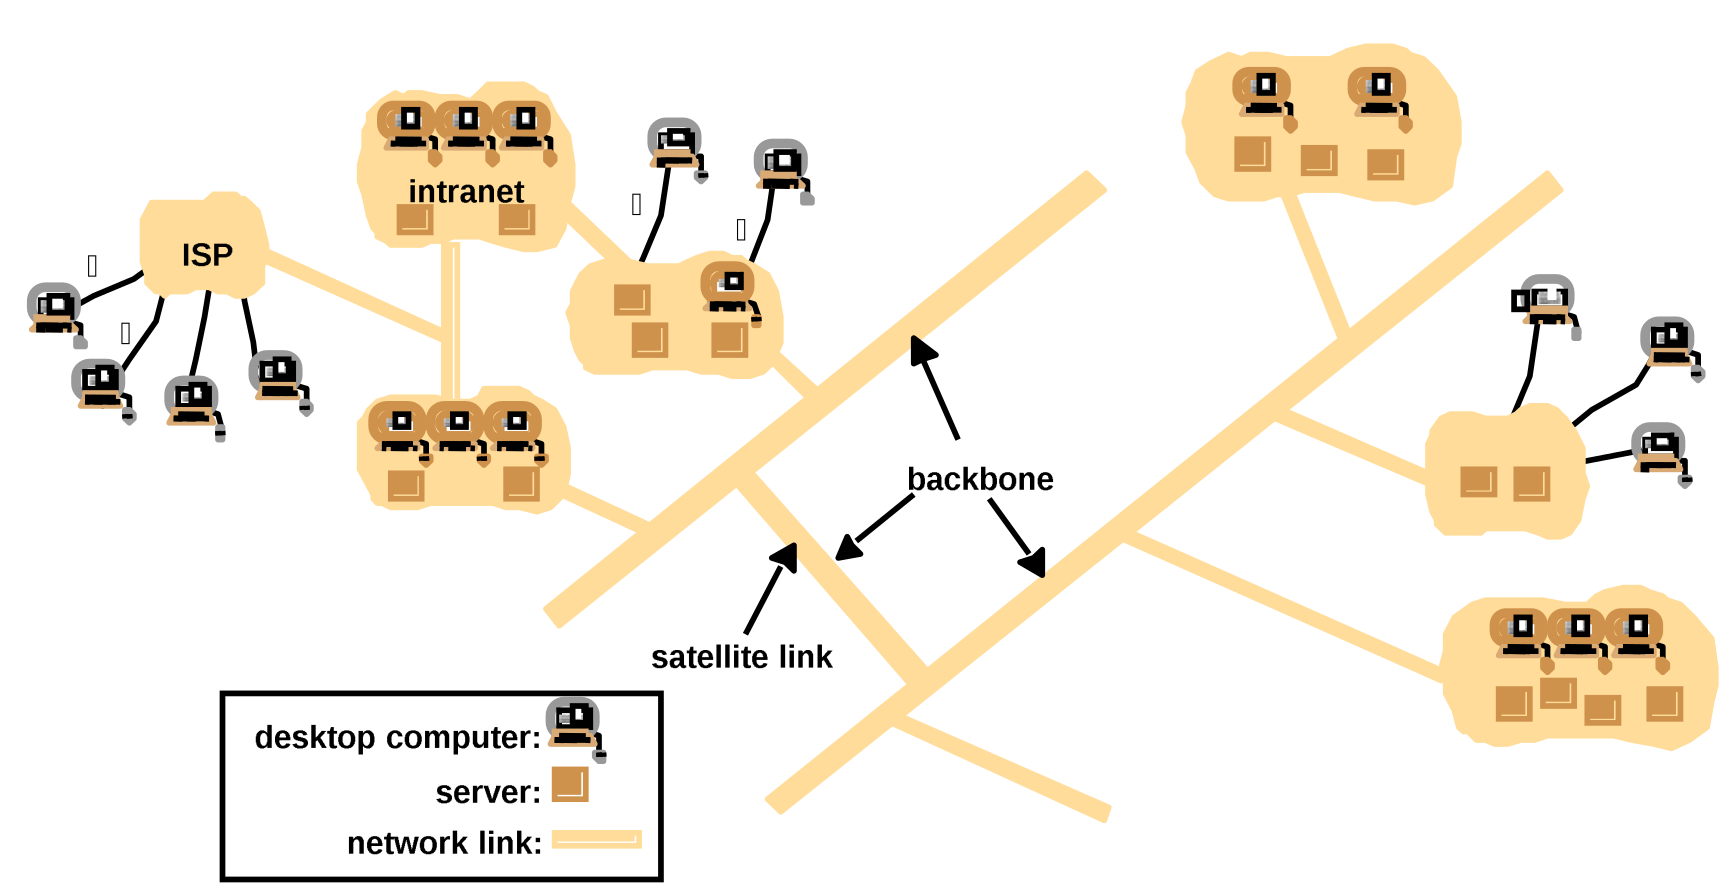
\includegraphics[scale=0.25]{figures/itsystem.png}
    \caption{Enterprise IT system \cite{Wong2014}}
    \label{fig:internet}
\end{figure}

Nowadays, most modern enterprise information systems are distributed systems, popularized due to the growth of the Internet.


Servers communicate with other servers using protocols, such as the HTTP protocol, based on the TCP/IP protocol. Communication can also happen locally (i.e., between computer processes, using interfaces such as sockets). Typically, such protocols are independent of the system architecture.

In fact, there are different architectures for organizing distributed systems. One of the simplest is the client-server architecture, where servers can expose endpoints to clients.
In this architecture, servers keep resources and serve those resources according to requests made by clients. Client-server architectures have a popularized programming model: RPC, and the more recent gRPC. Such protocols allow to structure distributed system programming, based on client calls on server's code. While this is an efficient scheme, it constitutes a centralized paradigm, that suffers from issues such as lack of scalability, and constitutes a single point of failure. Other architectures offer different tradeoffs: for instance, the peer-to-peer architecture is decentralized, which allows for a higher degree of openness, and fault tolerance. This makes the whole system more robust to faults. 

\subsection{Faults, Errors, and Failures}
A fault is an event that alters the normal behaviour of a system, which typically causes errors. Errors comprise the transition from a correct state of the system to an incorrect state. Errors can provoke failures, if the system deviates from its specification. The protection against faults allows participants to remain consistent: this way it is easier to maintain a correct state, that can be shared with other participants. Faults can be crash faults or byzantine faults. Crash faults are faults that make the system halt, for example, by creating network partitioning, or hardware problems. Typically, N nodes are capable to withstand up to $\frac{n}{2}$ crashes: crash fault tolerant (CFT) models can assume a quorum of $\frac{n}{2}+1$ nodes which has to agree on the global state. However, if one of the nodes are malicious, the system enters an faulty (or inconsistent) state. Faults caused by malicious actors are called Byzantine faults. Such faults are assumed when a system can behave arbitrarily (most difficult faults to resolve). Most byzantine-fault tolerant (BFT) algorithms need at least $3f+1$ honest nodes to support $f$ malicious nodes.

%figure client server vs distributed

But a question may arise: how to make sure that, in decentralized networks, the participants agree on a single state? How can we assure agreement under uncertain conditions, and assuming that participants can fail (e.g., connection problems)? What if there are malicious participants? This problem is also referred as the consensus problem, a well known problem studied the early stages of distributed systems.


\subsection{Consensus}
Consensus is a fundamental problem in distributed systems, in the area of fault tolerance. Consensus involves multiple server s (or nodes) agreeing on a global state (set of values). %The problem of consensus has been studied since the late 1970s, . 
The problem of reaching consensus was popularized by Pease, Shostak, and Lamport's Byzantine generals story, where the generals had to agree on a common plan to attack a city, where the messangers that exchanged their messages where unreliable \cite{byzantine_generals}.  

Distributed systems ought to be \emph{Byzantine fault-tolerant}, as there may be malicious nodes on the network \cite{correia2019byzantine}.  A consensus algorithm is used to create agreement on a global ledger state in the presence of crash faults or Byzantine faults. Consensus algorithms depend on the assumptions made about the environment and the system that the algorithm is running. For instance, what are the faults that can happen (crash vs byzantine), how are messages passed, synchronous (communication and processing delays are bounded) vs asynchronous (communication and processing delays are not bounded, i.e., may take an arbitrary amount of time to be completed) environment.

\subsection{State Machine Replication}
A general approach to building fault-tolerant systems is the state machine replication, that is studied in the context of consensus.  A state machine can be described by a set of possible initial states and next relation. This relation determines the possible steps, given the current step.

In a distributed system, each participating node has a state machine and a log. A log is a collection of log entries, which typically contain timestamped information. The state machine is a device (computer) that stores and manipulates state (e.g., values written in an hash table, the value of a variable, an array with commands to be executed). 

The idea of state machine replication is that clients can interact with a distributed system that agrees upon a global state, while it appears it is interacting with a single state machine. Even if one of the server fails, the system still responds to the requests. Each node takes commands from the logs, triggering the execution of a function. The consensus ensures that the commands received are the same; and ensures a common ordering for the commands received. This ensures that each state machine yields the same series of results, achieving the same series of states, at a common order. Each state machine executes the same function calls, in the same order, yielding the same output. For this reason, state machines need to be deterministic (otherwise, the same input could yield different outputs, causing inconsistencies in the system).
 
 \begin{figure}[h!]
    \centering
    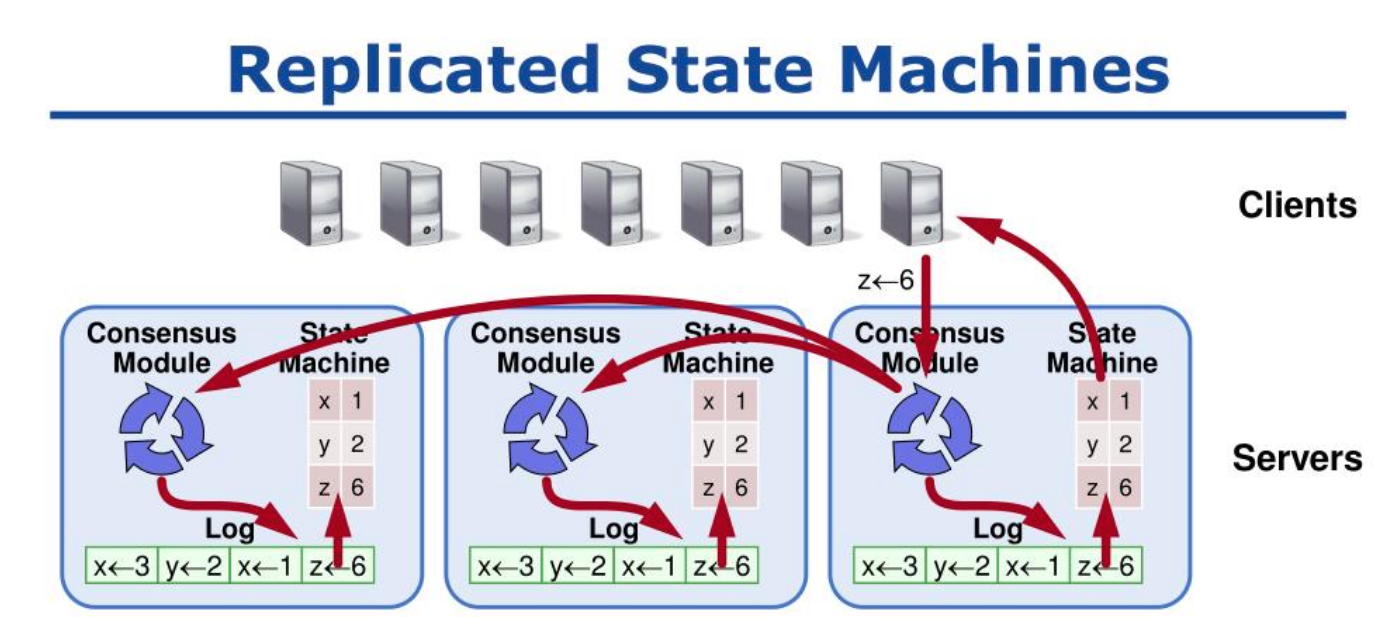
\includegraphics[scale=0.25]{figures/rsm.png}
    \caption{Replicated state machines \cite{replicated}}
    \label{fig:rms}
\end{figure}

Figure \ref{fig:rms} shows an example of a replicated state machine. A group of machines executes a deterministic function based on a replicated log they receive (input). The idea is that logs are kept identical so the execution on different machines is performed using the same commands, and on the same order. When the first machine receives an update request (set variable Z to 6), it first replicates that command into all the logs, passing that command to the other machines on the cluster. All machines add the newest command to the end of their logs. After that, the command can be executed by each state machine. This triggers the original state machine to return the answer of the execution to the client. If one of the servers (that comprises a state machine) fails, the other servers can still process the request, as far as a majority of servers are operational. There are consensus algorithms that allow to tolerating servers that crash (crash fault tolerant, CFT) or even servers that behave arbitrarily (e.g., malicious servers). The algorithms belonging to the latter category are called Byzantine fault tolerant (BFT). These systems allow to develop and deliver resilient, dependable systems that can satisfy today's needs in terms of availability and scalability.

With this in mind, consensus algorithms then aim to replicate commands into the replicated logs, allowing to assure desirable properties about a system: for example validity.

A system is valid if all correct processes that propose the same value, then any process decides that value. Moreover, a system is in agreement if no two correct processes decide differently (e.g., output different values for the same input). Termination is a liveness property, that states ``every correct process eventually decides". Those are all desirable properties for tolerant-fault systems. 

In this class, you will work in greater detail the RAFT algorithm: a well-adopted consensus algorithm, which focuses on understandability, and has many practical applications, inclusively on the blockchain area. 




 
\subsection{The RAFT consensus algorithm}

RAFT is a crash fault tolerant consensus algorithm that is designed to be easy to understand.  %Typically, crash fault tolerant leader-based algorithms have a linear message complexity, O(n), as opposed to Byzantine leader-based consensus, which incurrs in a quadratic message complexity (On2).  

It belongs to a class of consensus algorithms called leader-based (or coordinator-based or primary-backup). In leader-based consensus, there is a leader that calculates a decision on the state, and communicates it to the followers; if the leader is faulty, a new leader is elected.
RAFT considers several participants: 
\begin{itemize}
    \item Leader: the node that receives client requests, manages the log replication, and sends log update requests to other nodes. While having a leader that commands the global state is sufficient fine in some scenarios, a malicious leader can constitute a problem, as eventual inconsistencies are corrected (overwritten) by the leader.
    \item  Followers: constituting all nodes except the leader; 
    \item Candidates: followers requesting to be the leader.
\end{itemize}


As explained before, a distributed system built with RAFT has several servers running an instance of RAFT and a persistent log to store the commands received from clients. The replication of logs and consequent command execution is given by three phases:
\begin{enumerate}
    \item Leader Election
    \item Log Replication
    \item Safety
\end{enumerate}

Figure \ref{fig:state_empty} shows the global state, which corresponds to the state of each node (server), across the different terms (time periods in which the algorithm executes). Terms are used to detect obsolete information: there is at most one leader per term, and followers do not accept information coming from a previous term than the one they record. This way, the algorithm guarantees that each node has the latest information.

\begin{figure}
    \centering
    \subfloat[Initial state of the shared log of operations]{    \label{fig:state_empty}{\includegraphics[width=7cm]{figures/RAFT_state_empty.png} }}%
    \qquad
    \subfloat[Leader S2 received a command from a client. It wishes to updated state]{    \label{fig:RAFT5}{\includegraphics[width=7cm]{figures/RAFT_state.png} }}%
    \caption{States at different terms for each server}%
    \label{fig:state_empty}%
\end{figure}
 


\subsubsection{Leader Election}
Time in RAFT is divided into terms. Each terms has a unique identifier, a monotonically increasing number, which is set to 0 at server startup time. RAFT uses randomized timers to elect the leader, illustrated by Figure  \ref{fig:le_1}. At the beginning of the consensus process, nodes are awaiting for heartbeats from the leader (Figure \ref{fig:RAFT1}). When a follower receives a heartbeat, their timeouts are reset. As there is no leader, no heartbeats are received within the election timeout, and eventually a timeout is triggered. The node that triggered the timeout sends a proposal to become the new leader to every other node (Figure \ref{fig:RAFT2}), and eventually becomes the new leader.

If a node does not receive a heartbeat from a leader within a certain time frame (for example, in case the leader crashes), there is another timeout that initiates the beginning of a new term and a new leader election process starts.

\begin{figure}
    \centering
    \subfloat[There is no leader, each node awaits instructions]{    \label{fig:RAFT1}{\includegraphics[width=7cm]{figures/RAFT1.png} }}%
    \qquad
    \subfloat[After the timeout, the node sends a proposal to become the new leader]{    \label{fig:RAFT2}{\includegraphics[width=7cm]{figures/RAFT2.png} }}%
    \caption{Leader election process}%
    \label{fig:le_1}%
\end{figure}

The terms also allows for liveness: nodes reject requests coming with an invalid term number (older than the current term). Nodes ask to be a leader in a  first-come-first-served basis. As the majority rule applies, only one node can win an election and become the leader. In case of a draw, another round of election proceeds. Note that at the beginning of the execution, the log is empty (Figure \ref{fig:state_empty}).





\subsubsection{Log Replication}
The idea of log replication is the leader to accept requests from clients, which translate to commands that the server has to execute. Those commands are appended to a log. After that, the leader replicates its logs to other nodes on the network, so they can execute the received commands as well, in order to keep the states of all nodes consistent. Part of this procedure is illustrated by Figure \ref{fig:su_2}. 

Let us now suppose that a leader receives a request from a client (Figure \ref{fig:RAFT_state}). The log is updated, but it is still not safe to execute the received commands (as the log entry is considered uncommitted). This happens because followers are not aware of the request (illustrated by the dashed lines around an update). The leader broadcasts the most recent log entry to their followers, and receives a message from each one acknowledging that they received the updated log entry (Figure \ref{fig:RAFT6}). After the leader confirms the state, after receiving the acknowledgments from the followers, the followers can append the command to their logs, for later executing the command. 


\begin{figure}[h!]
    \centering
    \subfloat[Followers acknowledge the latest log entry]{    \label{fig:RAFT_state}{\includegraphics[width=7cm]{figures/RAFT5.png} }}%
    \qquad
    \subfloat[Global status is committed, that is, the received command from the client is present in the logs of the majority of nodes, so each node can now execute it]{    \label{fig:RAFT6}{\includegraphics[width=7cm]{figures/RAFT6.png} }}%
    \caption{State updates}%
    \label{fig:su_2}%
\end{figure}

Imagine that now, node S2 crashes due to a hardware fail. This causes that S2 cannot send heartbeats back to each follower. We now assume that S1 timeouts - it becomes a candidate and tries to become a leader (Figure \ref{fig:crash}). When a follower becomes a candidate, it increments the current term, votes for itself, and send requests to other followers, to become the new leader. Eventually, S1 wins the election and becomes the new leader (Figure \ref{fig:new_leader}).

\begin{figure}[h!]
    \centering
    \subfloat[Server S2 crashes. A follower triggers a timeout, becoming a candidate. The candidate S1 tries to become the leader]{    \label{fig:crash}{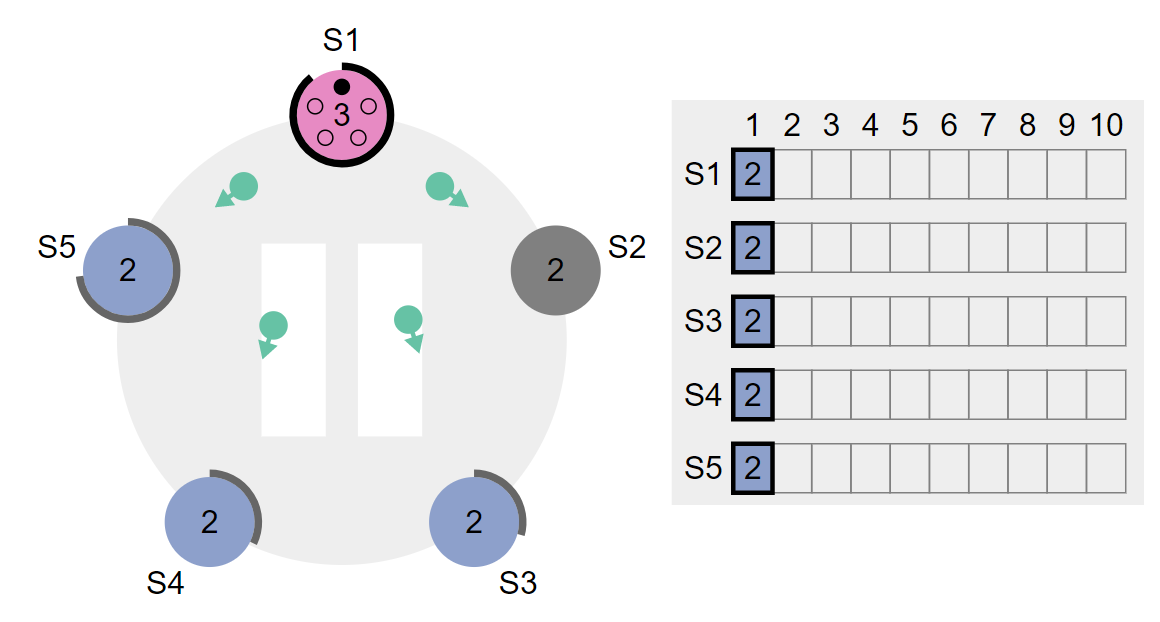
\includegraphics[width=7cm]{figures/s2_crash.png} }}%
    \qquad
    \subfloat[Candidate S1 becomes the leader]{    \label{fig:new_leader}{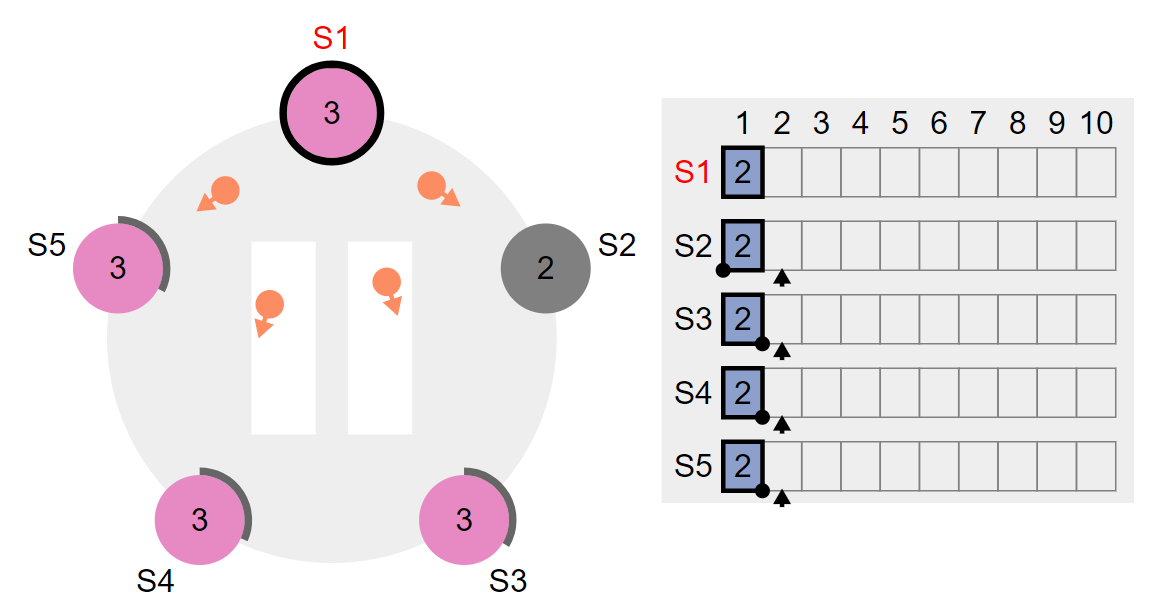
\includegraphics[width=7cm]{figures/new_leader.PNG} }}%
    \caption{New leader election process}%
    \label{fig:leader_election}%
\end{figure}


\subsubsection{Safety}
Logs need to be kept consistent, and, furthermore, that only nodes with the latest log version can become leaders. 
If a crash occurs, log inconsistencies may happen. In other words, the information stored by each node may not be the same at the same point. To solve this problem, the log of the current leader is always considered the correct version. The leader repairs inconsistencies, if applicable. For that, there cannot be missing log entries, and log entries need to be ordered.

RAFT's approach to maintain consistency is by matching logs and solving conflicts: each time a leader sends a log entry to a follower, it includes the term number and log index of the preeceding entry. If there is a match, the follower accepts the new log entry; otherwise, the follower rejects the log entry. In case a log entry is rejected, the leader tries again, sending the current log entry, the preceeding one, and the one further before., until a match happens. When a match happens, the follower's log is updated, accordingly to the leader.


The explained mechanisms guarantee the log matching property: if a given entry is committed, all previous entries are committed and, if two logs share the same log index and term, then those logs are identical (represent the same log entry). Lastly, the desirable safety tackles leader completeness: once a log entry is committed, the leader will have that log entry stored. This assures a committed entry is never lost. Nodes with incomplete logs are not chosen in the election process. Essentially, a node denies the vote if their log is more complete than the candidate's log.


\section{Hands on RAFT}
Now, that we illustrated the RAFT algorithm, let's consolidate that knowledge. It is recommended for students to read the additional support materials available: \cite{raft_paper,raft_homepage}. You may use the simulator provided at RAFT's homepage to aid you in your responses\footnote{https://RAFT.github.io/}.


\subsubsection*{Exercise 1:} To consolidate your knowledge, watch the a guided visualization of the RAFT algorithm \cite{raft_viz}. 
Elaborate on how the RAFT algorithm can contribute to increase the availability of the system, from a client perspective.

\subsubsection*{Exercise 2:} When does a new term start? 



\subsubsection*{Exercise 3:} How does candidates act if two of them attempt to become leaders at exactly the same time?


\subsubsection*{Exercise 4:} If a follower receives a message has a different term than the one recorded, doeos it accept the message?  

\subsubsection*{Exercise 5:} Suppose that a leader receives a command from a client, and notifies all followers. Upon sending the second transaction, one of the followers crashes. How does RAFT guarantee that the follower is updated?



\subsubsection*{Exercise 6:} Consider the following RAFT cluster, composed by a leader and four followers. The leader has sent eight messages, corresponding to eight commands. Those eight commands translate into eight log entries. The current term is term three. 
\begin{figure}[H]
    \centering
    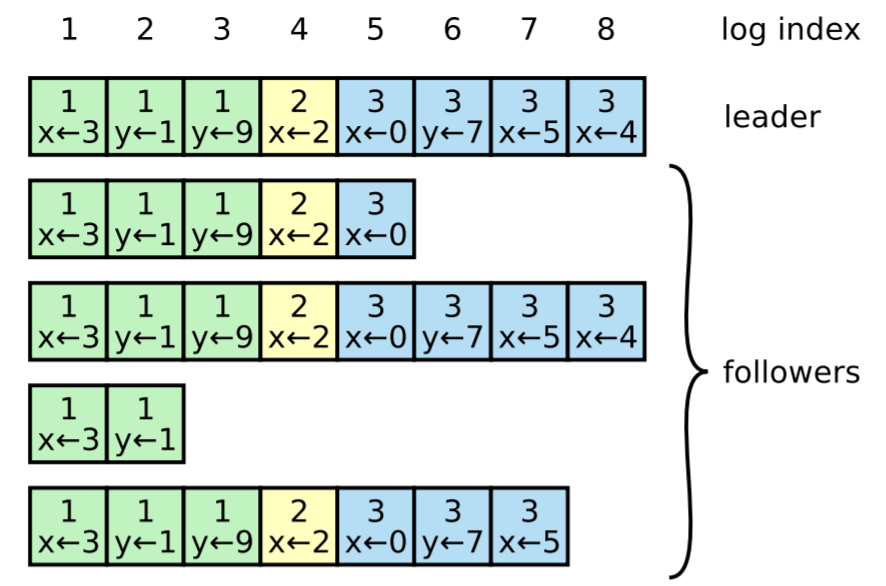
\includegraphics[scale=0.6]{figures/exercise.png}
    \caption{RAFT cluster composed of 5 machines}
    \label{fig:RAFT_cluster}
\end{figure}

What are the commands, represented by each log index, that are safe to be executed by each node?

\subsubsection*{Exercise 7:} Consider the following RAFT cluster, composed by a leader and four followers, in which there are inconsistencies on the logs across nodes. Assume that node S4 crashed on term 1. Node S5 became the leader on term 2, but was only successful to replicate logs 4 and 5, before crashing. Node S3 is the leader on term 3.

\begin{figure}[H]
    \centering
    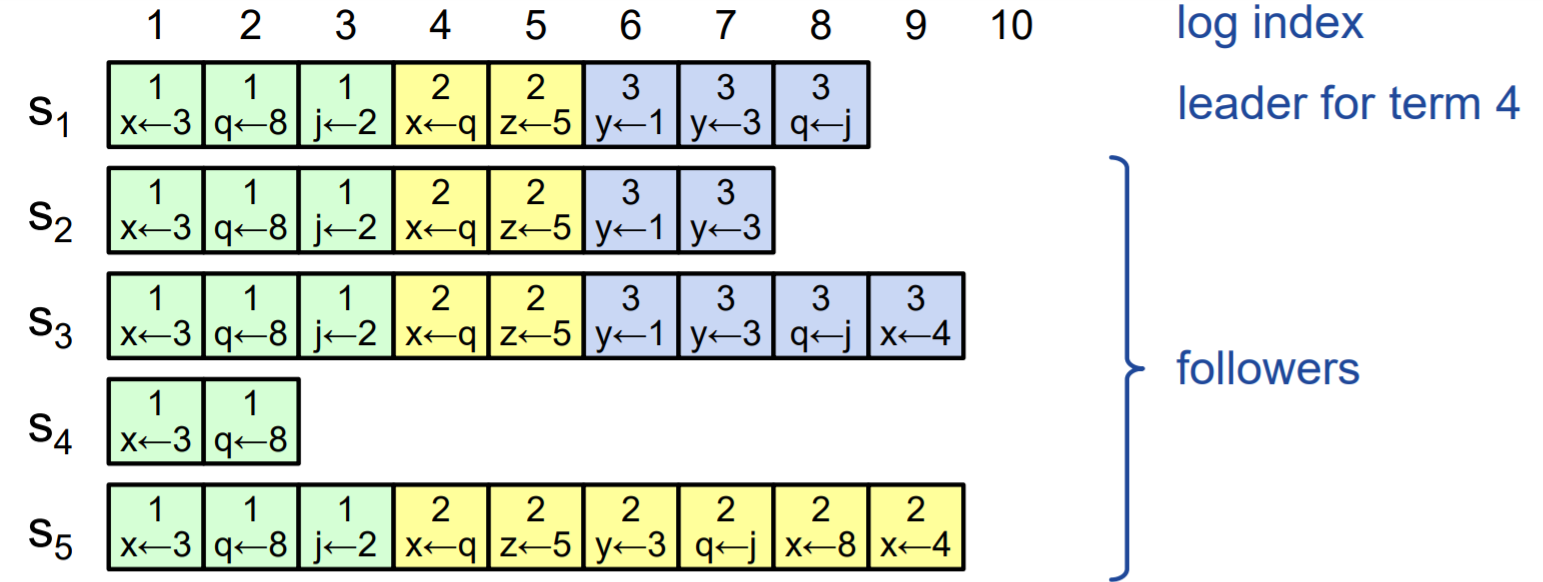
\includegraphics[scale=0.6]{figures/inconsistent_logs.png}
    \caption{RAFT cluster composed of 5 servers, showing inconsistencies regarding the log}
    \label{fig:inconsistent_logs}
\end{figure}

What will be the final state of the system, assuming no new commands are received, and that S5 recovers from crash?


\subsubsection*{Exercise 8:} During the leader election process, a mechanism that ensure consistency across logs is the rejection of candidates that have outdated logs. What are the checks the follower does against the candidate's proposal? In which occasion does it reject voting on the candidate?


\subsubsection*{Exercise 9:} Consider the following RAFT cluster, composed by seven nodes.

\begin{figure}[H]
    \centering
    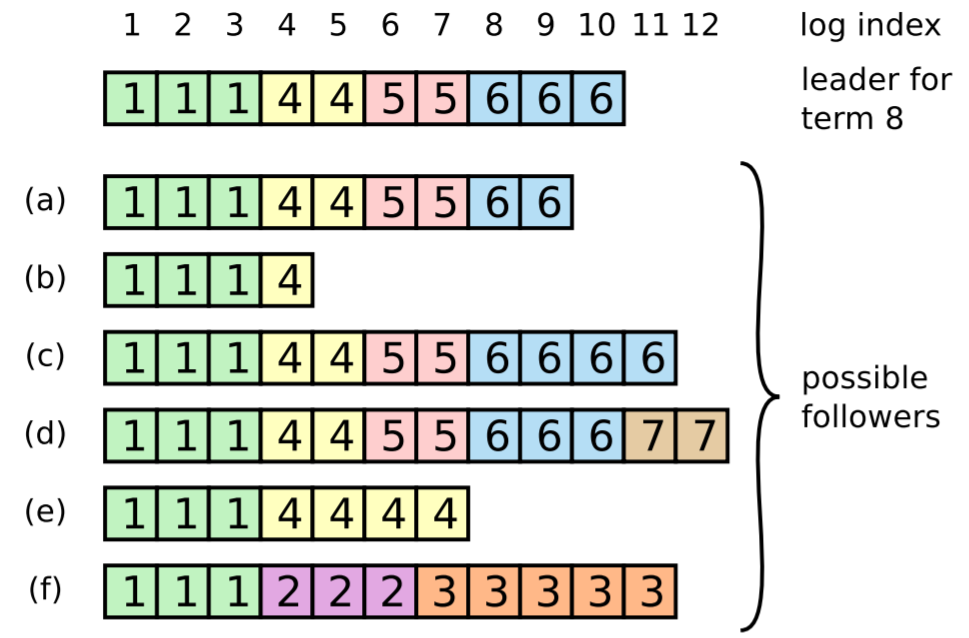
\includegraphics[scale=0.6]{figures/discussion.png}
    \caption{RAFT cluster composed of 7 nodes}
    \label{fig:inconsistent_logs}
\end{figure}

Given that the leader of term eight has ten log entries, and interacts with six followers, how did the system get into this state?

\subsubsection*{Exercise 10:} How does the system re-organize itself if a node leaves the system?


%%%%%%%%%%%%%%%%%%%%%%%%%%%%%%%%%%%%%%%%%%%%%%%%%%%%%%%%%%%%%%%%%%%%%%%%%%%%%%%%%%%
% YOUR TEXT ENDS HERE
%%%%%%%%%%%%%%%%%%%%%%%%%%%%%%%%%%%%%%%%%%%%%%%%%%%%%%%%%%%%%%%%%%%%%%%%%%%%%%%%%%% 
\bibliographystyle{IEEEtran}
\bibliography{lab1.bib}

\end{document}                             % The required last line